\documentclass[a4paper,12pt]{article}

\author{Cy Baca}

% comments
\usepackage{multicol}
\usepackage{xcolor}
\usepackage{graphicx}

\begin{document}

\begin{center}
    \Large{\textbf{Gaussian Elimination Assignment}} \\
    \small{\textbf{by Cy Baca}} \\
\end{center}

\section{How your program stores the data}
    All of the matrix data used by the program is stored in a global struct
    variable called \texttt{\_vectors}, which holds pointers to doubles to:

        \begin{itemize}
        \item \texttt{*echelon}, the matrix to perform reduction on
        \item \texttt{*variables}, an array to hold the x values during back
              substitution
        \item \texttt{*original}, a copy of the values that were generated at
              the beginning of the program
        \item \texttt{**rows}, an array of pointers to doubles which reprsent
              the location of the beginning of each row in the echelon matrix.
        \end{itemize}

    All of the arrays in \texttt{\_vectors} are allocated contiguously and
    aligned to the \emph{cache line size} of the given architecture by making
    calls to \texttt{posix\_memalign()} and \texttt{sysconf()}, in order to reduce
    the chance of threads pulling overlapping cache lines.

    There is one more global struct variable called \texttt{\_stats}, but it is
    only used at the beginning and end of the program to store and print
    benchmark data. All other variables during runtime are created and used
    within, or passed to and from, functions.

\section{How your program partitions the data and work and exploits parallelism}

    The program can be broken down into a series of stages.
    \begin{itemize}
    \item\emph{Initialization}
    \item\emph{Gaussian Elimination}
        \begin{itemize}
        \item\emph{Matrix Reduction(parallel)}
        \item\emph{Back substitution(parallel)}
        \item\emph{L2 Norm}
        \end{itemize}
    \item\emph{Finalization}
    \end{itemize}

    Each stage is define by a function, or group of functions, with names that represent
    its purpose. Functions that are part of a certain stage have the first part of their
    master function's name with an underscore appended to the front of them so that their
    purpose is easy to determine just from reading the name. For example, the
    \emph{Matrix Reduction} stage starts with \texttt{echelon\_reduce()} and
    every function that is directly or indirectly used by it are prefixed with
    "\texttt{\_echelon\_<etc>}".

    \subsection*{Initialization}
    The first stage, \emph{initialization},  begins in \texttt{main()} by
    checking args for \textbf{"N"}, and passing the \textbf{N} value to \texttt{program\_init()}.
    From there, \texttt{\_vectors} is passed by reference to
    \texttt{vectors\_init()}, where a series of functions initializes the
    pointers with heap memory, and initializes the memory pointed to by
    \texttt{original} with random doubles from -1.0e6 to 1.0e6, and copies that
    memory over to \texttt{echelon}.

    \subsection*{Gaussian Elimination}
    The data is passed to \texttt{gaussian\_elimination()}, where all of the major
    matrix math functions are called in a specific order, starting with
    \texttt{echelon\_reduce()}

    \texttt{echelon\_reduce()} and each of its helper functions act as a
    series of nested \emph{for} loops and loop nests, but are broken down into
    functions. I chose this strategy for two reason:
    \begin{itemize}
    \item To keep the pattern of data mutation concise and manageable.
    \item To make clear and seperate sections of parallelized code.
    \end{itemize}
    \subsection*{Back substitution}
    When \texttt{echelon\_reduce()} is finished, it returns to
    \texttt{gaussian\_elimination()}, after which \texttt{back\_substitution()}
    is called. This section uses a two level nested for loop and employs a
    slighlty different strategy than the last.
    This time, the threads all share a given row, and work on it at the same
    time. When the row is complete, the threads enter a critical section and
    write to the \texttt{variable} array. This way, the chances of reading from
    a dirty piece of memory while retrieving the next \emph{x} value is
    mitigated.

    \subsection*{L2 Norm}
    This section is not parallelized, and it used to validate the approximated
    x values. If the L2 Norm is not a very low number, there is likey an error
    in the previous calculations.

    \subsection*{Finalization}
    Finally, the benchmark values are printed to the console, and all heap
    memory used at runtime is deleted.

    \subsection*{Parallel sections:}
    \begin{itemize}
    \item in \texttt{\_echelon\_pivot()} for finding the next pivot. Each row gets
          a chunk of the current diagonal column and searches for the largest value
          at each index. Afterward, the threads meet at a critical section where
          they largest index is stored in a shared variable.
    \item in \texttt{\_echelon\_annihilation()}. Each row gets a private pointer to the beginning
          of its own row, finds its own multiplier, and reduces that row. This
          allows threads to simulatneously read data from the pivot row needed by each of
          them. Meanwhile, each thread is guaranteed to be the only thread with
          a copy of its write data for all rows with a length greater than the
          cache line size.
    \item in \texttt{back\_substitution()}, where the parallel section starts on the inner
    loop of a double nested \emph{for} loop. This means, that multiple threads share a row.
    In order to compensate for possible cache line discrepencies, I used a dynamic schedule with
    the parameter of the \texttt{l1d cache\_line\_size / sizeof(double)}. This way, threads should
    have chunk sizes with data that no other thread contains, avoiding false sharing.
    \end{itemize}


\section{How the parallel work is synchronized}

    In \texttt{echelon\_eliminate()}, in the annihilation loop, the default
    schedule is used, (meaning it should be static, with chunks the size of
    the ratio loop length to threads). The only private variable is the
    pointer pointer used to iterate through the row indexes, and there are
    seven shared variables.

    In the \emph{Partial Pivoting} parallel section, the default schedule is
    used again for the \emph{for} loop, which divides a column up by chunks of
    indices. This time, the threads share two variables: one for reducing the
    largest value in the column, and one for storing its index. Within the
    section, each thread finds the highest value within its chunk, and then
    enters a critical section. Since I couldn't figure out how to make a
    directive that would synchronize a reduction for a max value \textbf{and}
    store the index, I had to explicitly create a \emph{critical} section where
    the threads could compare max values, and write if needed.

    In the \emph{Back Substitution} section, I tried opened a parallel section
    using the reduction(-) directive for each X value. I first used the \emph{guided}
    schedule to try to accomodate for the growing size of the rows, but didn't see
    improvement. I ended up using \emph{dynamic} with size 8 (cache line size / sizeof(double)
    which shaved off a few seconds, although the default \emph{static} schedule seemed to
    work equally as well.

\section{Pseudocode that sketches the key elements of your parallelization strategy}

    If all of the main matrix maths functions where concatenated into one function, it
    would likely look something like the following:

    \begin{verbatim}

    /** start **/
    number_of_pivots = N - 1

    double **rows =  { pointer to beginning of each row }

    foreach cur_pivot_index in rows, cur_row < number_of_pivots

        next_pivot_index = 0;

        /* partial pivot **********************************/

        #parallel section

            start = cur_row[0]

            for index in column_under_start

                reduce(max(column_under_start[index]))

                #critical

                    next_pivot_index = index

            swap(rows[cur_pivot_index], rows[next_pivot_index])

        /* annihilation **********************************/
        pivot = &rows[cur_row][next_pivot_index]

        #parallel for
        for cur_row in rows + 1

            cur_multiplier = cur_row / pivot[0]

            for i in row

                cur_row[i] -= multiplier * pivot[i]

    /* back substitution **********************************/
    foreach last_index in rows, --last_index

        next_variable

        cur_row = &(*rows)[last_index]

        #parallel for private(next_variable) reduction(-)
        foreach upper_triangle_index in cur_row

            next_variable -= cur_row[upper_triangle_index] *
            variables[upper_trianlge_index]

        variables[last_index] = next_variable /
        cur_row[upper_triangle_index];

    \end{verbatim}


\section{Your justification for your implementation choices}

    I originally wrote the entire program without the partial pivoting section,
    because I had overlooked that part of the assignment(oops). This influenced
    the outcome of my program design decisions, for better or for worse, in how
    I ended up allocating memory, loop structure, and mechanisms for iterating
    over the data.

    \begin{description}
    \item Before implementing partial pivoting:

        I wanted to use contiguous memory so that I could
        \begin{itemize}
        \item keep it aligned to a cache block
        \item maintain tight spacial locality
        \end{itemize}

    \item After realizing I needed to implement partial pivoting I needed to figure
        out a way to iterate over the contiguous memory in a specific order without
        incurring too much overhead.
        
    \item So, I ended using a pointer to an array of pointers.

        I malloc'd a pointer to an array of double pointers, and pointer
        each one at indexes corresponding to the beginning of the rows in
        my original contiguous \texttt{echelon} array. Even though I eneded up
        with a 2D array, I used it as a reference point for other pointers
        to iterate over rows in \emph{for} loops; then, when partial pivoting
        was around the corner(ha ha, no pun intended), I could just swap the
        pointers in the pointer array, and by annihilation time I had a way
        to iterate in the correct order without any extra fuss.
    \end{description}

    I don't know how much, if any, extra overhead was caused by the extra pointer
    variables I needed to add for loop iterations, in contrast to just instatiating
    my data in 2D array from the beginning, and I didn't have a chance to try
    this implementation, so it remains a mystery.

    I do know that I drastically overestimated the overhead cost of implementing
    the partial pivoting section of the code, because I didn't notice much(a second
    or two if anything) change in timing from before I implented it, so that part
    was a success.


\section{How successful your approach was}
        
        My setup was very marginally successful. For two two threads, I got a
        fat speedup increase from 0.0 to 1.8, with an efficiecy of 9.1. After
        that, the efficiency was neraly halved to 0.56, and this pattern
        continued all the way up to 40 cores, where I ended up with less tham
        0.08 efficiency.

        I imagine the lack of efficiency must be at least partially due to the
        scalability of the problem itself. Many of the operations that need to
        take place for Gaussian Elimination rely on the completion of previous
        operations on the data before they can carry on. This means that there
        is limited space for threads to work concurrently.

        Considering that the parallelization of the code required only \emph{six}
        lines of code, I really impressed with the amount of speedup I was able
        to squeeze out of it. I don't want to imagine the nightmare I'd have to
        endure trying to complete the same work using posix threads or the cold
        hard futex library.

        All in all, I guess my approach was at least marginally successful.


\section{Table of the time to execute and the l2-norm, for every run, with the
   minimum time on p cores highlighted}

\begin{center}
\begin{tabular}{| l | l | l | l} \hline
    threads: & times: & l2norms: \\ \hline

    1 & \begin{tabular}{l} 664.261893 \\ 724.946826 \\ \colorbox{yellow}{654.247888}\\ \end{tabular} &
    \begin{tabular}{l} 2.5800157282e-03 \\ 9.4443812796e-04 \\ 9.0724052356e-03 \\ 
    \end{tabular} \\ \hline

    2 &
    \begin{tabular}{l} 365.474405 \\  \colorbox{yellow}{360.074551}  \\  501.253396 \\ \end{tabular} &
    \begin{tabular}{l} 4.5947765776e-04 \\ 3.0701745230e-04 \\ 6.6478362796e-04 \\
    \end{tabular} \\ \hline

    5 &
    \begin{tabular}{l} \colorbox{yellow}{230.183935}  \\ 232.148950 \\ 411.946127 \\ \end{tabular} &
    \begin{tabular}{l} 2.1035538762e-04 \\ 1.1235548047e-03 \\  1.5833014563e-03 \\
    \end{tabular} \\ \hline

    10 &
    \begin{tabular}{l} 219.263489 \\ \colorbox{yellow}{219.164048}  \\ 219.367498 \\ \end{tabular} &
    \begin{tabular}{l} 2.1327824368e-04 \\ 1.1445531847e-03 \\ 1.2088836573e-03 \\
    \end{tabular} \\ \hline

    20 &
    \begin{tabular}{l} \colorbox{yellow}{214.652390}  \\ 404.893739 \\ 214.777489 \\ \end{tabular} &
    \begin{tabular}{l}
    1.3031318008e-03 \\ 3.0483806989e-04 \\ 9.3423978678e-04 \\ \end{tabular} \\ \hline

    30 &
    \begin{tabular}{l} 213.484887 \\ 213.462830 \\ \colorbox{yellow}{213.336266} \\ \end{tabular} &
    \begin{tabular}{l}
    4.7350450144e-04 \\ 3.1031698941e-03 \\ 4.1833982675e-04 \\ 
    \end{tabular} \\ \hline

    40 &
    \begin{tabular}{l} \colorbox{yellow}{413.856779} \\ 215.757580 \\ 214.470610 \\ \end{tabular} &
    \begin{tabular}{l}
    3.1035303350e-04 \\ 5.5170123099e-04 \\ 1.8542336495e-03  \\
    \end{tabular} \\ \hline
\end{tabular}
\end{center}


\section{Table of the minimum times, calculated speedup, efficiency, l2-norm}

\begin{center}
\begin{tabular}{| l | l | l | l |} \hline
    threads: & minimum time: & speedup: & efficiency\\ \hline
1 & 654.247888 & 0.0 & 1.0 \\ \hline
2 & 360.074551 & 1.816979 & 0.908489 \\ \hline
5 & 230.183935 & 2.842283 & 0.568457 \\ \hline
10 & 219.164048 & 2.985197 & 0.298520 \\ \hline
20 & 214.652390 & 3.047941 & 0.152397 \\ \hline
30 & 213.336266 & 3.066745 & 0.102225 \\ \hline
40 & 214.470610 & 3.050525 & 0.076263 \\ \hline
\end{tabular}
\end{center}


\section{Separate graphs of speedup and efficiency}
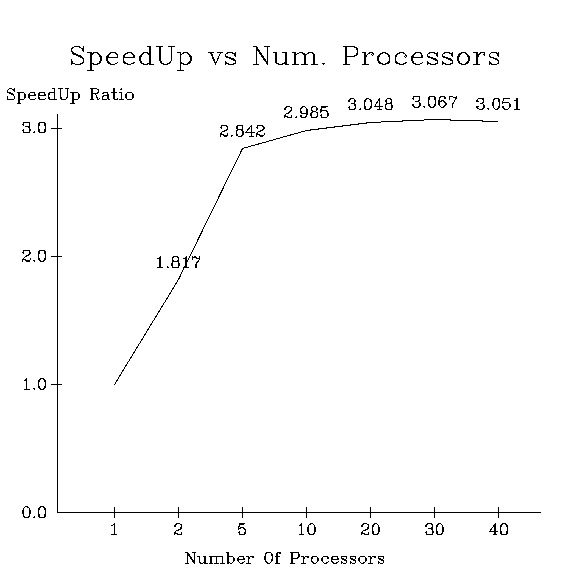
\includegraphics[scale=0.75]{./speedup.png} \\
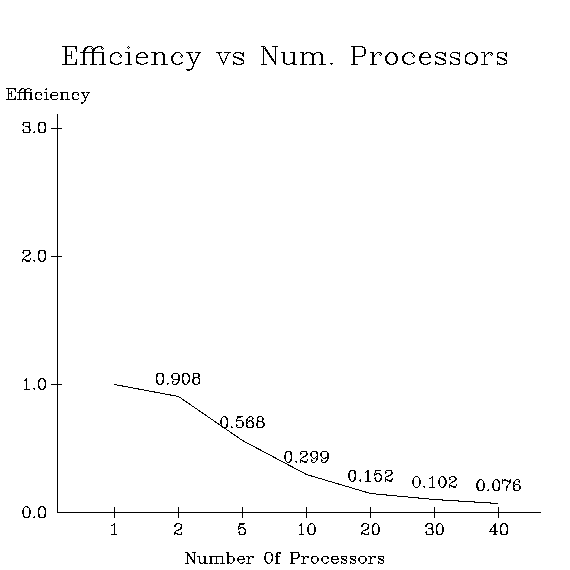
\includegraphics[scale=0.75]{./efficiency.png}

\end{document}
